
\documentclass[runningheads,a4]{llncs}
\usepackage{amssymb}
\setcounter{tocdepth}{3}
\usepackage[dvipdfmx]{graphicx}
\usepackage{tikz}
\usepackage{amsmath}

\usetikzlibrary{automata}
\usetikzlibrary{arrows}
\usetikzlibrary{positioning}
\usepackage{here}
\usepackage{enumitem}
\usepackage{wrapfig}
\usetikzlibrary{decorations.markings}
\DeclareMathOperator*{\argmin}{arg\,min}

\usetikzlibrary{lindenmayersystems}
\bibliographystyle{junsrt}

\usepackage{url}
\urldef{\mailsa}\path|{s.skei@uec.ac.jp|
\newcommand{\keywords}[1]{\par\addvspace\baselineskip
\noindent\keywordname\enspace\ignorespaces#1}
\begin{document}
%---------------------------
\subsection{Turner}
%---------------------------
Turner consists of two parts, bit bifurcator and steering arm (colored in yellow in Figure~\ref{over_all}).
%steering arm
Steering arm changes the route by AO



\begin{figure}[H]
  \begin{tabular}{c}
 
  
  \begin{minipage}{0.5\hsize}
  \centering
  \scalebox{0.5}{
  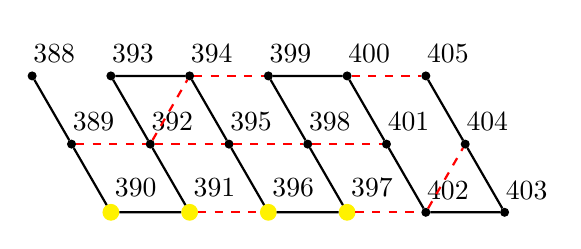
\begin{tikzpicture}[node distance=1cm,every node/.style={draw,circle,fill,inner sep=1pt}]
   \node[yellow,inner sep = 2pt] (3) at (0:0)[label=above right:390]{};
  \node (2) at (120:1)[label=above right:389]{};
  \node (1)at (120:2)[label=above right:388]{};
  \node[right of= 1] (6) [label=above right:393]{};
  \node[right of =6](7)[label=above right:394]{};
  \node[right of =7](12)[label=above right:399]{};
\node[right of =12](13)[label=above right:400]{};
\node[right of =13](18)[label=above right:405]{};
  \node[right of =2](5)[label=above right:392]{};
  \node[right of =5](8)[label=above right:395]{};
  \node[right of =8](11)[label=above right:398]{};
\node[right of =11](14)[label=above right:401]{};
\node[right of =14](17)[label=above right:404]{};
  \node[right of =3,yellow,inner sep = 2pt](4)[label=above right:391]{};
  \node[right of =4,yellow,inner sep = 2pt](9)[label=above right:396]{};
  \node[right of =9,yellow,inner sep = 2pt](10)[label=above right:397]{};
\node[right of =10](15)[label=above right:402]{};
\node[right of =15](16)[label=above right:403]{};
%\node[above =1.6cm of  5,fill = green,inner sep = 2pt](100){};
  \draw[thick](1)--(2)--(3)--(4)--(5)--(6)--(7)--(8)--(9)--(10)--(11)--(12)--(13)--(14)--(15)--(16)--(17)--(18);
  \draw[dashed,thick,red](2)--(5);
  \draw[dashed,thick,red](5)--(8);
  \draw[dashed,thick,red](4)--(9);
  \draw[dashed,thick,red](5)--(7);
  %\draw[dashed,thick,red](6)--(100);
  %\draw[dashed,thick,red](7)--(100);
  \draw[dashed,thick,red](7)--(12);
  \draw[dashed,thick,red](8)--(11);
  \draw[dashed,thick,red](11)--(14);
  \draw[dashed,thick,red](10)--(15);
  \draw[dashed,thick,red](13)--(18);
  \draw[dashed,thick,red](15)--(17);
  \end{tikzpicture}
  }

  \end{minipage}

 \begin{minipage}{0.5\hsize}
  \centering
  \scalebox{0.5}{
  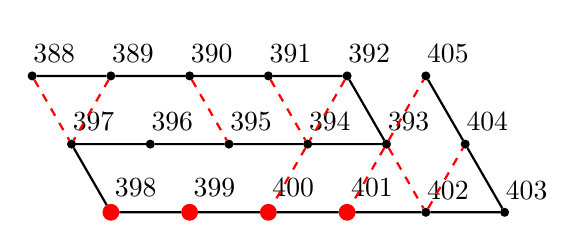
\begin{tikzpicture}[node distance=1cm,every node/.style={draw,circle,fill,inner sep=1pt}]
  \node [red,inner sep = 2pt] (11) at (0:0)[label=above right:398]{};
  \node (10) at (120:1)[label=above right:397]{};
  \node (1)at (120:2)[label=above right:388]{};
  \node[right of= 1] (2) [label=above right:389]{};
  \node[right of =2](3)[label=above right:390]{};
  \node[right of =3](4)[label=above right:391]{};
  \node[right of =4](5)[label=above right:392]{};
  \node[right of =5](18)[label=above right:405]{};
  \node[right of =10](9)[label=above right:396]{};
  \node[right of =9](8)[label=above right:395]{};
  \node[right of =8](7)[label=above right:394]{};
  \node[right of =7](6)[label=above right:393]{};
  \node[right of =6](17)[label=above right:404]{};
  \node[right of =11,red,inner sep = 2pt](12)[label=above right:399]{};
  \node[right of =12,red,inner sep = 2pt](13)[label=above right:400]{};
  \node[right of =13,red,inner sep = 2pt](14)[label=above right:401]{};
  \node[right of =14](15)[label=above right:402]{};
  \node[right of =15](16)[label=above right:403]{};
%\node[above =1.6cm of 9,fill = green,inner sep = 2pt](100){};
  \draw[thick](1)--(2)--(3)--(4)--(5)--(6)--(7)--(8)--(9)--(10)--(11)--(12)--(13)--(14)--(15)--(16)--(17)--(18);
  %\draw[dashed,thick,red](2)--(100);
  %\draw[dashed,thick,red](2)--(100);
  \draw[dashed,thick,red](1)--(10);
  \draw[dashed,thick,red](2)--(10);
  \draw[dashed,thick,red](3)--(8);
  \draw[dashed,thick,red](4)--(7);
  \draw[dashed,thick,red](5)--(7);
  \draw[dashed,thick,red](7)--(13);
  \draw[dashed,thick,red](6)--(14);
  \draw[dashed,thick,red](6)--(15);
  \draw[dashed,thick,red](6)--(18);
  \draw[dashed,thick,red](15)--(17);
  \end{tikzpicture}
  }
 
  \end{minipage}

  \end{tabular}
  \caption{body-rpx1(T-A)のカンファメーション2つ、body-gx(T-E)とbody-gx'(T-F)の下にあるやつ、左がT-A0,右がT-A1、T-A0での393と394の間の上のビーズから情報を得ている}
\label{body-px}
\end{figure} 
%%%%%%%%%%%%%%%%%%%%%%%%%%%%%%%%%%%%%%%%%%%%%%%%%%%%%%%%%%%%%%%%%%%%%%%%%%%%%%%%%%%%%%%%%%%%%%%%%%%%%%%%%%%%%%%%%%%

\begin{figure}[H]
  \begin{tabular}{c}
 
  
  \begin{minipage}{0.5\hsize}
  \centering
  \scalebox{0.5}{
  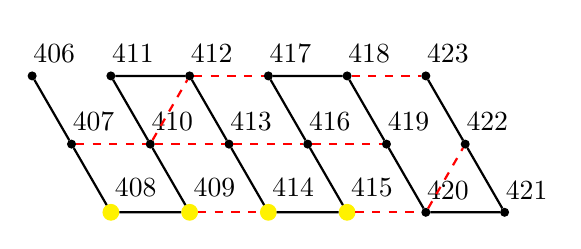
\begin{tikzpicture}[node distance=1cm,every node/.style={draw,circle,fill,inner sep=1pt}]
   \node[yellow,inner sep = 2pt] (3) at (0:0)[label=above right:408]{};
  \node (2) at (120:1)[label=above right:407]{};
  \node (1)at (120:2)[label=above right:406]{};
  \node[right of= 1] (6) [label=above right:411]{};
  \node[right of =6](7)[label=above right:412]{};
  \node[right of =7](12)[label=above right:417]{};
\node[right of =12](13)[label=above right:418]{};
\node[right of =13](18)[label=above right:423]{};
  \node[right of =2](5)[label=above right:410]{};
  \node[right of =5](8)[label=above right:413]{};
  \node[right of =8](11)[label=above right:416]{};
\node[right of =11](14)[label=above right:419]{};
\node[right of =14](17)[label=above right:422]{};
  \node[right of =3,yellow,inner sep = 2pt](4)[label=above right:409]{};
  \node[right of =4,yellow,inner sep = 2pt](9)[label=above right:414]{};
  \node[right of =9,yellow,inner sep = 2pt](10)[label=above right:415]{};
\node[right of =10](15)[label=above right:420]{};
\node[right of =15](16)[label=above right:421]{};
%\node[above =1.6cm of  5,fill = green,inner sep = 2pt](100){};
  \draw[thick](1)--(2)--(3)--(4)--(5)--(6)--(7)--(8)--(9)--(10)--(11)--(12)--(13)--(14)--(15)--(16)--(17)--(18);
  \draw[dashed,thick,red](2)--(5);
  \draw[dashed,thick,red](5)--(8);
  \draw[dashed,thick,red](4)--(9);
  \draw[dashed,thick,red](5)--(7);
  %\draw[dashed,thick,red](6)--(100);
  %\draw[dashed,thick,red](7)--(100);
  \draw[dashed,thick,red](7)--(12);
  \draw[dashed,thick,red](8)--(11);
  \draw[dashed,thick,red](11)--(14);
  \draw[dashed,thick,red](10)--(15);
  \draw[dashed,thick,red](13)--(18);
  \draw[dashed,thick,red](15)--(17);
  \end{tikzpicture}
  }

  \end{minipage}

 \begin{minipage}{0.5\hsize}
  \centering
  \scalebox{0.5}{
  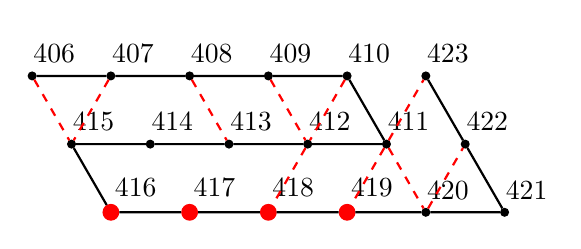
\begin{tikzpicture}[node distance=1cm,every node/.style={draw,circle,fill,inner sep=1pt}]
  \node [red,inner sep = 2pt] (11) at (0:0)[label=above right:416]{};
  \node (10) at (120:1)[label=above right:415]{};
  \node (1)at (120:2)[label=above right:406]{};
  \node[right of= 1] (2) [label=above right:407]{};
  \node[right of =2](3)[label=above right:408]{};
  \node[right of =3](4)[label=above right:409]{};
  \node[right of =4](5)[label=above right:410]{};
  \node[right of =5](18)[label=above right:423]{};
  \node[right of =10](9)[label=above right:414]{};
  \node[right of =9](8)[label=above right:413]{};
  \node[right of =8](7)[label=above right:412]{};
  \node[right of =7](6)[label=above right:411]{};
  \node[right of =6](17)[label=above right:422]{};
  \node[right of =11,red,inner sep = 2pt](12)[label=above right:417]{};
  \node[right of =12,red,inner sep = 2pt](13)[label=above right:418]{};
  \node[right of =13,red,inner sep = 2pt](14)[label=above right:419]{};
  \node[right of =14](15)[label=above right:420]{};
  \node[right of =15](16)[label=above right:421]{};
%\node[above =1.6cm of 9,fill = green,inner sep = 2pt](100){};
  \draw[thick](1)--(2)--(3)--(4)--(5)--(6)--(7)--(8)--(9)--(10)--(11)--(12)--(13)--(14)--(15)--(16)--(17)--(18);
  %\draw[dashed,thick,red](2)--(100);
  %\draw[dashed,thick,red](2)--(100);
  \draw[dashed,thick,red](1)--(10);
  \draw[dashed,thick,red](2)--(10);
  \draw[dashed,thick,red](3)--(8);
  \draw[dashed,thick,red](4)--(7);
  \draw[dashed,thick,red](5)--(7);
  \draw[dashed,thick,red](7)--(13);
  \draw[dashed,thick,red](6)--(14);
  \draw[dashed,thick,red](6)--(15);
  \draw[dashed,thick,red](6)--(18);
  \draw[dashed,thick,red](15)--(17);
  \end{tikzpicture}
  }
 
  \end{minipage}

  \end{tabular}
  \caption{body-rpx2(T-B)のカンファメーション2つ、body-lpx2(T-D)の下にあるやつ、左がT-B0,右がT-B1、情報を得ているビーズはT-Aと一緒}
\label{body-px}
\end{figure} 





%%%%%%%%%%%%%%%%%%%%%%%%%%%%%%%%%%%%%%%%%%%%%%%%%%%%%%%%%%%%%%%%%%%%%%%%%%%%%%%%%%%%%%%%%%%%%%%%%%%%%%%%%%%%%%%%%%%

\begin{figure}[H]
  \begin{tabular}{c}
 
  
  
  
  \begin{minipage}{0.5\hsize}
  \centering
  \scalebox{0.5}{
  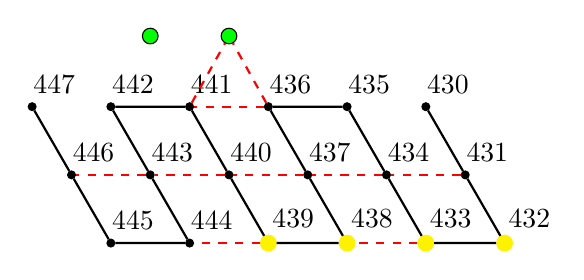
\begin{tikzpicture}[node distance=1cm,every node/.style={draw,circle,fill,inner sep=1pt}]
   \node[yellow,inner sep = 2pt] (3) at (0:0)[label=above right:432]{};
  \node (2) at (120:1)[label=above right:431]{};
  \node (1)at (120:2)[label=above right:430]{};
  \node[left of= 1] (6) [label=above right:435]{};
  \node[left of =6](7)[label=above right:436]{};
  \node[left of =7](12)[label=above right:441]{};
\node[left of =12](13)[label=above right:442]{};
\node[left of =13](18)[label=above right:447]{};
  \node[left of =2](5)[label=above right:434]{};
  \node[left of =5](8)[label=above right:437]{};
  \node[left of =8](11)[label=above right:440]{};
\node[left of =11](14)[label=above right:443]{};
\node[left of =14](17)[label=above right:446]{};
  \node[left of =3,yellow,inner sep = 2pt](4)[label=above right:433]{};
  \node[left of =4,yellow,inner sep = 2pt](9)[label=above right:438]{};
  \node[left of =9,yellow,inner sep = 2pt](10)[label=above right:439]{};
\node[left of =10](15)[label=above right:444]{};
\node[left of =15](16)[label=above right:445]{};
\node[above =1.6cm of  11,fill = green,inner sep = 2pt](100){};
\node[above =1.6cm of  14,fill = green,inner sep = 2pt](101){};
  \draw[thick](1)--(2)--(3)--(4)--(5)--(6)--(7)--(8)--(9)--(10)--(11)--(12)--(13)--(14)--(15)--(16)--(17)--(18);
  \draw[dashed,thick,red](2)--(5);
  \draw[dashed,thick,red](5)--(8);
  \draw[dashed,thick,red](8)--(11);
  \draw[dashed,thick,red](11)--(14);
  \draw[dashed,thick,red](14)--(17);
  \draw[dashed,thick,red](4)--(9);
  \draw[dashed,thick,red](7)--(12);
  \draw[dashed,thick,red](10)--(15);
  \draw[dashed,thick,red](7)--(100);
  \draw[dashed,thick,red](12)--(100);
  \end{tikzpicture}
  }
  \end{minipage}

 \begin{minipage}{0.5\hsize}
  \centering
  \scalebox{0.5}{
  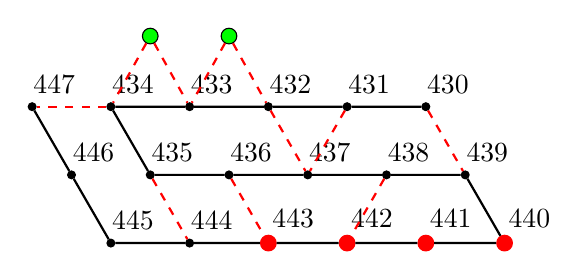
\begin{tikzpicture}[node distance=1cm,every node/.style={draw,circle,fill,inner sep=1pt}]
  \node [red,inner sep = 2pt] (11) at (0:0)[label=above right:440]{};
  \node (10) at (120:1)[label=above right:439]{};
  \node (1)at (120:2)[label=above right:430]{};
  \node[left of= 1] (2) [label=above right:431]{};
  \node[left of =2](3)[label=above right:432]{};
  \node[left of =3](4)[label=above right:433]{};
  \node[left of =4](5)[label=above right:434]{};
  \node[left of =5](18)[label=above right:447]{};
  \node[left of =10](9)[label=above right:438]{};
  \node[left of =9](8)[label=above right:437]{};
  \node[left of =8](7)[label=above right:436]{};
  \node[left of =7](6)[label=above right:435]{};
  \node[left of =6](17)[label=above right:446]{};
  \node[left of =11,red,inner sep = 2pt](12)[label=above right:441]{};
  \node[left of =12,red,inner sep = 2pt](13)[label=above right:442]{};
  \node[left of =13,red,inner sep = 2pt](14)[label=above right:443]{};
  \node[left of =14](15)[label=above right:444]{};
  \node[left of =15](16)[label=above right:445]{};
\node[above =1.6cm of 6,fill = green,inner sep = 2pt](100){};
\node[above =1.6cm of 7,fill = green,inner sep = 2pt](101){};
  \draw[thick](1)--(2)--(3)--(4)--(5)--(6)--(7)--(8)--(9)--(10)--(11)--(12)--(13)--(14)--(15)--(16)--(17)--(18);
  \draw[dashed,thick,red](1)--(10);
  \draw[dashed,thick,red](2)--(8);
  \draw[dashed,thick,red](3)--(8);
  \draw[dashed,thick,red](9)--(13);
  \draw[dashed,thick,red](7)--(14);
  \draw[dashed,thick,red](6)--(15);
  \draw[dashed,thick,red](5)--(18);
  \draw[dashed,thick,red](100)--(5);
  \draw[dashed,thick,red](100)--(4);
  \draw[dashed,thick,red](101)--(4);
  \draw[dashed,thick,red](101)--(3);
  \end{tikzpicture}
  }
  \end{minipage}
 
\\

  
  \end{tabular}
  \caption{%body-lpx2
body-lpx1(T-C)のカンファメーション2つ、body-rpx1(T-A)の下にあるやつ、左がT-C0,右がT-C1、%%T-A0での393と394の間の上のビーズから情報を得ている
}
\label{body-px}
\end{figure} 





%%%%%%%%%%%%%%%%%%%%%%%%%%%%%%%%%%%%%%%%%%%%%%%%%%%%%%%%%%%%%%%%%%%%%%%%%%%%%%%%%%%%%%%%%%%%%%%%%%%%%%%%%%%%%%%%
\begin{figure}[H]
  \begin{tabular}{c}
 

  \begin{minipage}{0.5\hsize}
  \centering
  \scalebox{0.5}{
  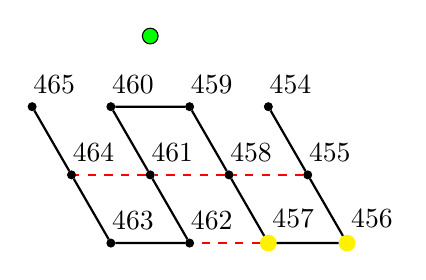
\begin{tikzpicture}[node distance=1cm,every node/.style={draw,circle,fill,inner sep=1pt}]
  \node (3) at (0:0) [yellow,inner sep =2pt,label=above right:456]{};
  \node (2) at (120:1)[label=above right:455]{};
  \node (1)at (120:2)[label=above right:454]{};
  \node[left of= 1] (6) [label=above right:459]{};
  \node[left of =6](7)[label=above right:460]{};
  \node[left of =7](12)[label=above right:465]{};
  \node[left of =2](5)[label=above right:458]{};
  \node[left of =5](8)[label=above right:461]{};
  \node[left of =8](11)[label=above right:464]{};
  \node[left of =3](4)[yellow,inner sep = 2pt,label=above right:457]{};
  \node[left of =4,](9)[label=above right:462]{};
  \node[left of =9](10)[label=above right:463]{};
  

\node[above =1.6cm of  8,fill = green,inner sep = 2pt](100){};
  \draw[thick](1)--(2)--(3)--(4)--(5)--(6)--(7)--(8)--(9)--(10)--(11)--(12);
  \draw[dashed,thick,red](2)--(5);
  \draw[dashed,thick,red](5)--(8);
  \draw[dashed,thick,red](8)--(11);
  \draw[dashed,thick,red](4)--(9);
  \end{tikzpicture}
  }
  
  \end{minipage}

 \begin{minipage}{0.5\hsize}
  \centering
  \scalebox{0.5}{
  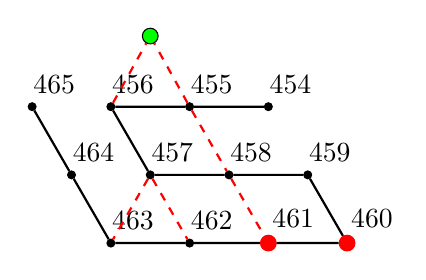
\begin{tikzpicture}[node distance=1cm,every node/.style={draw,circle,fill,inner sep=1pt}]
  \node (7) at (0:0)[red,inner sep = 2pt,label=above right:460]{};
  \node (6) at (120:1)[label=above right:459]{};
  \node (1)at (120:2)[label=above right:454]{};
  \node[left of= 1] (2) [label=above right:455]{};
  \node[left of =2](3)[label=above right:456]{};
  \node[left of =3](12)[label=above right:465]{};
  \node[left of =6](5)[label=above right:458]{};
  \node[left of =7,red,inner sep = 2pt](8)[label=above right:461]{};
  \node[left of =8](9)[label=above right:462]{};
  \node[left of =9](10)[label=above right:463]{};
  \node[left of =5](4)[label=above right:457]{};
  \node[left of =4](11)[label=above right:464]{};
  
\node[above =1.6cm of 4,fill = green,inner sep = 2pt](100){};

  \draw[thick](1)--(2)--(3)--(4)--(5)--(6)--(7)--(8)--(9)--(10)--(11)--(12);
  \draw[dashed,thick,red](2)--(5);
  \draw[dashed,thick,red](5)--(8);
  \draw[dashed,thick,red](4)--(9);
  \draw[dashed,thick,red](4)--(10);
  \draw[dashed,thick,red](2)--(100);
  \draw[dashed,thick,red](3)--(100);
  \end{tikzpicture}
  }
  
  \end{minipage}
  \end{tabular}
  \caption{%body-lpx2
body-lpx2(T-D)のカンファメーション2つ、body-gx1(T-E)とbody-gx2(T-F)の下にあるやつ、左がT-D0,右がT-D1、}
\label{body-px}
\end{figure} 

%%%%%%%%%%%%%%%%%%%%%%%%%%%%%%%%%%%%%%%%%%%%%%%%%%%%%%%%%%%%%%%%%%%%%%%%%%%%%%%%%%%%%%%%%%%%%%
	\begin{figure}[H]
  \begin{tabular}{c}
  \begin{minipage}{0.25\hsize}
  \centering
  \scalebox{0.5}{
  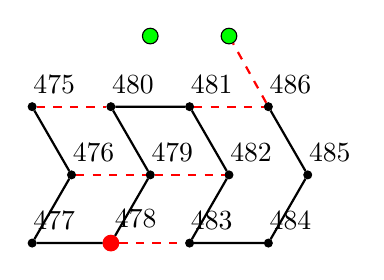
\begin{tikzpicture}[node distance=1cm,every node/.style={draw,circle,fill,inner sep=1pt}]
  \node (3) at (0:0)[label=above right:477]{};
  \node (2) at (60:1)[label=above right:476]{};
  \node (6)at (60:2)[label=above right:480]{};
  \node[right of =3,red,inner sep = 2pt](4)[label=above right:478]{};
  \node[right of =4](9)[label=above right:483]{};
  \node[right of =9](10)[label=above right:484]{};
  
  \node[right of =2](5)[label=above right:479]{};
  \node[right of =5](8)[label=above right:482]{};
  \node[right of =8](11)[label=above right:485]{};
  
  \node[left of= 6] (1) [label=above right:475]{};
  \node[right of =6](7)[label=above right:481]{};
  \node[right of =7](12)[label=above right:486]{};
  \node[above =1.6cm of 8,fill = green,inner sep = 2pt](100){};
  \node[above =1.6cm of 5,fill = green,inner sep = 2pt](101){};
  \draw[thick](1)--(2)--(3)--(4)--(5)--(6)--(7)--(8)--(9)--(10)--(11)--(12);
  \draw[dashed,thick,red](1)--(6);
  \draw[dashed,thick,red](2)--(5);
  \draw[dashed,thick,red](4)--(9);
  \draw[dashed,thick,red](5)--(8);
  \draw[dashed,thick,red](7)--(12);
  \draw[dashed,thick,red](12)--(100);
  \end{tikzpicture}
  }
  
  \end{minipage}

\begin{minipage}{0.25\hsize}
  \centering
  \scalebox{0.5}{
  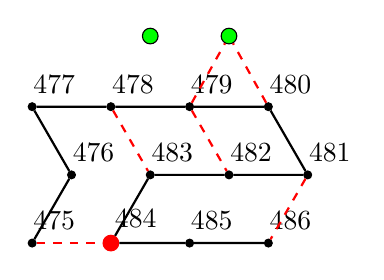
\begin{tikzpicture}[node distance=1cm,every node/.style={draw,circle,fill,inner sep=1pt}]
  \node (1) at (0:0)[label=above right:475]{};
  \node (2) at (60:1)[label=above right:476]{};
  \node (4)at (60:2)[label=above right:478]{};
  \node[left of= 4] (3) [label=above right:477]{};
  \node[right of =4](5)[label=above right:479]{};
    \node[right of =5](6)[label=above right:480]{};
    \node[right of =2](9)[label=above right:483]{};
    \node[right of =9](8)[label=above right:482]{};
    \node[right of =8](7)[label=above right:481]{};
    \node[right of =1,red,inner sep = 2pt](10)[label=above right:484]{};
    \node[right of =10](11)[label=above right:485]{};
    \node[right of =11](12)[label=above right:486]{};
  
  \node[above =1.6cm of 8,fill = green,inner sep = 2pt](100){};
\node[above =1.6cm of 9,fill = green,inner sep = 2pt](101){};
  \draw[thick](1)--(2)--(3)--(4)--(5)--(6)--(7)--(8)--(9)--(10)--(11)--(12);
  \draw[dashed,thick,red](4)--(9);
  \draw[dashed,thick,red](5)--(8);
  \draw[dashed,thick,red](7)--(12);
  \draw[dashed,thick,red](1)--(10);
  \draw[dashed,thick,red](5)--(100);
  \draw[dashed,thick,red](6)--(100);
  \end{tikzpicture}
  }
 
  \end{minipage}

\begin{minipage}{0.25\hsize}
  \centering
  \scalebox{0.5}{
  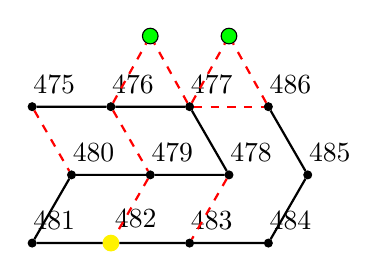
\begin{tikzpicture}[node distance=1cm,every node/.style={draw,circle,fill,inner sep=1pt}]
  \node (1) at (0:0)[label=above right:475]{};
  \node (6) at (-60:1)[label=above right:480]{};
  \node (8)at (-60:2)[yellow,inner sep = 2pt,label=above right:482]{};
 \node[left of= 8] (7) [label=above right:481]{};
  \node[right of =1](2)[label=above right:476]{};
  \node[right of =2](3)[label=above right:477]{};
  \node[right of =6](5)[label=above right:479]{};
  \node[right of =5](4)[label=above right:478]{};
  \node[right of =8](9)[label=above right:483]{};
  \node[right of =9](10)[label=above right:484]{};
  \node[right of =3](12)[label=above right:486]{};
  \node[right of =4](11)[label=above right:485]{};
  
 
  \node[above =1.6cm of 4,fill = green,inner sep = 2pt](100){};
\node[above =1.6cm of 5,fill = green,inner sep = 2pt](101){};
  
  \draw[thick](1)--(2)--(3)--(4)--(5)--(6)--(7)--(8)--(9)--(10)--(11)--(12);
  \draw[dashed,thick,red](1)--(6);
  \draw[dashed,thick,red](2)--(5);
  \draw[dashed,thick,red](5)--(8);
  \draw[dashed,thick,red](4)--(9);
  \draw[dashed,thick,red](3)--(12);
  \draw[dashed,thick,red](2)--(101);
  \draw[dashed,thick,red](3)--(101);
  \draw[dashed,thick,red](3)--(100);
  \draw[dashed,thick,red](12)--(100);
  \end{tikzpicture}
  }
  
  \end{minipage}


\begin{minipage}{0.25\hsize}
  \centering
  \scalebox{0.5}{
  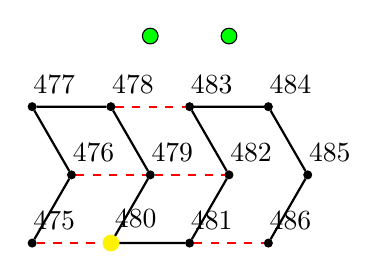
\begin{tikzpicture}[node distance=1cm,every node/.style={draw,circle,fill,inner sep=1pt}]
  \node (3) at (0:0)[label=above right:477]{};
  \node (2) at (-60:1)[label=above right:476]{};
  \node (6)at (-60:2)[yellow,inner sep = 2pt,label=above right:480]{};
  \node[right of =3](4)[label=above right:478]{};
  \node[right of =4](9)[label=above right:483]{};
  \node[right of =9](10)[label=above right:484]{};
  
  \node[right of =2](5)[label=above right:479]{};
  \node[right of =5](8)[label=above right:482]{};
  \node[right of =8](11)[label=above right:485]{};
  
  \node[left of= 6] (1) [label=above right:475]{};
  \node[right of =6](7)[label=above right:481]{};
  \node[right of =7](12)[label=above right:486]{};

  \node[above =1.6cm of 8,fill = green,inner sep = 2pt](){};
\node[above =1.6cm of 5,fill = green,inner sep = 2pt](){};
  \draw[thick](1)--(2)--(3)--(4)--(5)--(6)--(7)--(8)--(9)--(10)--(11)--(12);
  \draw[dashed,thick,red](1)--(6);
  \draw[dashed,thick,red](7)--(12);
  \draw[dashed,thick,red](2)--(5);
  \draw[dashed,thick,red](5)--(8);
  \draw[dashed,thick,red](4)--(9);
  \end{tikzpicture}
  }
 
  \end{minipage}
  \end{tabular}
  \caption{body-gx(T-E)のカンファメーション4つ、body-rpx1(T-A)とbody-lpx1(T-C)の下にあるやつ、左からT-E0,T-E1,T-E2,T-E3}
\label{body-gx}
\end{figure} 

%%%%%%%%%%%%%%%%%%%%%%%%%%%%%%%%%%%%%%%%%%%%%%%%%%%%%%%%%%%%%%%%%%%%%%%%%%%%%%%%%%%%%%%%%%%%%%%%%%%%%%%%%%%%%%


\begin{figure}[H]
  \begin{tabular}{c}
  \begin{minipage}{0.25\hsize}
  \centering
  \scalebox{0.5}{
  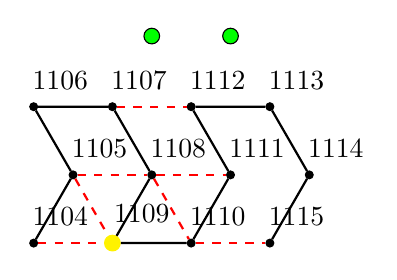
\begin{tikzpicture}[node distance=1cm,every node/.style={draw,circle,fill,inner sep=1pt}]
  \node (4) at (0:0)[label=above right:1104]{};
  \node (5) at (60:1)[label=above right:1105]{};
  \node (7)at (60:2)[label=above right:1107]{};

  \node[right of =4,yellow,inner sep = 2pt](9)[label=above right:1109]{};
  \node[right of =9](10)[label=above right:1110]{};
  \node[right of =10](15)[label=above right:1115]{};


  \node[right of =5](8)[label=above right:1108]{};
  \node[right of =8](11)[label=above right:1111]{};
  \node[right of =11](14)[label=above right:1114]{};
  
  \node[left of= 7] (6) [label=above right:1106]{};

  \node[right of =7](12)[label=above right:1112]{};
  \node[right of =12](13)[label=above right:1113]{};
  
  \node[above =1.6cm of 8,fill = green,inner sep = 2pt](){};
  \node[above =1.6cm of 11,fill = green,inner sep = 2pt](){};
  \draw[thick](4)--(5)--(6)--(7)--(8)--(9)--(10)--(11)--(12)--(13)--(14)--(15);
  \draw[dashed,thick,red](5)--(8);
  \draw[dashed,thick,red](5)--(9);
  \draw[dashed,thick,red](4)--(9);
  \draw[dashed,thick,red](8)--(11);
  \draw[dashed,thick,red](8)--(10);
  \draw[dashed,thick,red](7)--(12);
  \draw[dashed,thick,red](10)--(15);
  \end{tikzpicture}
  }
  %\caption*{上から0、横と下方向に0}
  \end{minipage}

\begin{minipage}{0.25\hsize}
  \centering
  \scalebox{0.5}{
  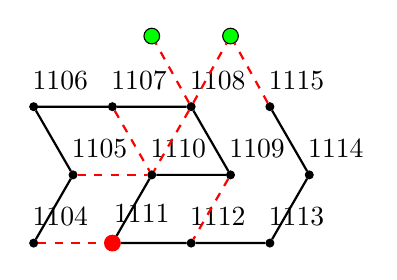
\begin{tikzpicture}[node distance=1cm,every node/.style={draw,circle,fill,inner sep=1pt}]
  \node (4) at (0:0)[label=above right:1104]{};
  \node (5) at (60:1)[label=above right:1105]{};
  \node (7)at (60:2)[label=above right:1107]{};
  \node[left of= 7] (6) [label=above right:1106]{};

    \node[right of =7](8)[label=above right:1108]{};
    \node[right of =8](15)[label=above right:1115]{};


    \node[right of =5](10)[label=above right:1110]{};
    \node[right of =10](9)[label=above right:1109]{};
    \node[right of =9](14)[label=above right:1114]{};

    \node[right of =4,red,inner sep = 2pt](11)[label=above right:1111]{};
    \node[right of =11](12)[label=above right:1112]{};
    \node[right of =12](13)[label=above right:1113]{};

  
  \node[above =1.6cm of 9,fill = green,inner sep = 2pt](100){};
\node[above =1.6cm of 10,fill = green,inner sep = 2pt](101){};
  \draw[thick](4)--(5)--(6)--(7)--(8)--(9)--(10)--(11)--(12)--(13)--(14)--(15);
  \draw[dashed,thick,red](5)--(10);
  \draw[dashed,thick,red](7)--(10);
  \draw[dashed,thick,red](8)--(10);
  \draw[dashed,thick,red](4)--(11);
  \draw[dashed,thick,red](9)--(12);
  \draw[dashed,thick,red](8)--(100);
  \draw[dashed,thick,red](8)--(101);
  \draw[dashed,thick,red](15)--(100);
  \end{tikzpicture}
  }
  %\caption*{上から1、横と下方向に1}
  \end{minipage}

 % \end{tabular}
 % \caption{body-rgy}
%\label{body-rgy}
%\end{figure} 


%	\begin{figure}[H]
  %\begin{tabular}{c}
  \begin{minipage}{0.25\hsize}
  \centering
  \scalebox{0.5}{
  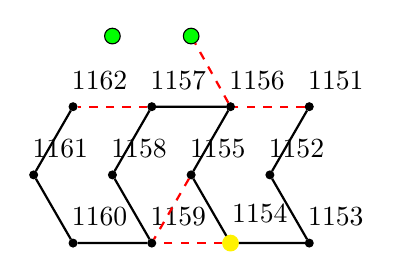
\begin{tikzpicture}[node distance=1cm,every node/.style={draw,circle,fill,inner sep=1pt}]
  \node (9) at (0:0)[label=above right:1153]{};
  \node (8) at (120:1)[label=above right:1152]{};
  \node (12)at (120:2)[label=above right:1156]{};


  \node[left of =9,yellow,inner sep = 2pt](10)[label=above right:1154]{};
  \node[left of =10](15)[label=above right:1159]{};
  \node[left of =15](16)[label=above right:1160]{};
  
  \node[left of =8](11)[label=above right:1155]{};
  \node[left of =11](14)[label=above right:1158]{};
  \node[left of =14](17)[label=above right:1161]{};
  
  \node[right of= 12](7)[label=above right:1151]{};

  \node[left of =12](13)[label=above right:1157]{};
  \node[left of =13](18)[label=above right:1162]{};
  \node[above =1.6cm of 14,fill = green,inner sep = 2pt](){};
  \node[above =1.6cm of 11,fill = green,inner sep = 2pt](100){};
  \draw[thick](7)--(8)--(9)--(10)--(11)--(12)--(13)--(14)--(15)--(16)--(17)--(18);
  \draw[dashed,thick,red](7)--(12);
  \draw[dashed,thick,red](10)--(15);
  \draw[dashed,thick,red](11)--(15);
  \draw[dashed,thick,red](13)--(18);
  \draw[dashed,thick,red](12)--(100);
  \end{tikzpicture}
  }
  %\caption*{上から0、横と下方向に0}
  \end{minipage}

\begin{minipage}{0.25\hsize}
  \centering
  \scalebox{0.5}{
  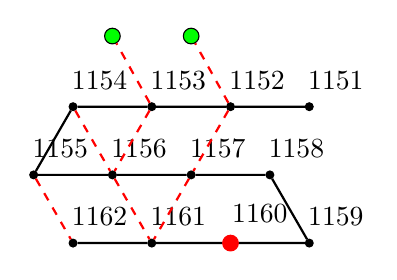
\begin{tikzpicture}[node distance=1cm,every node/.style={draw,circle,fill,inner sep=1pt}]
   \node (15) at (0:0)[label=above right:1159]{};
  \node (14) at (120:1)[label=above right:1158]{};
  \node (8)at (120:2)[label=above right:1152]{};

  \node[right of= 8] (7) [label=above right:1151]{};


  \node[left of =8](9)[label=above right:1153]{};
  \node[left of =9](10)[label=above right:1154]{};
  \node[left of =14](13)[label=above right:1157]{};
  \node[left of =13](12)[label=above right:1156]{};
  \node[left of =12](11)[label=above right:1155]{};

  \node[left of =15,red,inner sep = 2pt](16)[label=above right:1160]{};
  \node[left of =16](17)[label=above right:1161]{};
  \node[left of =17](18)[label=above right:1162]{};
 
  \node[above =1.6cm of 12,fill = green,inner sep = 2pt](100){};
\node[above =1.6cm of 13,fill = green,inner sep = 2pt](101){};
  \draw[thick](7)--(8)--(9)--(10)--(11)--(12)--(13)--(14)--(15)--(16)--(17)--(18);
  \draw[dashed,thick,red](8)--(13);
  \draw[dashed,thick,red](9)--(12);
  \draw[dashed,thick,red](10)--(12);
  \draw[dashed,thick,red](13)--(17);
  \draw[dashed,thick,red](12)--(17);
  \draw[dashed,thick,red](11)--(18);
  \draw[dashed,thick,red](8)--(101);
  \draw[dashed,thick,red](9)--(100);
  \end{tikzpicture}
  }
  %\caption*{上から1、横と下方向に1}
  \end{minipage}

  \end{tabular}
  \caption{%body-lgy
left:body-rgy,right:body-lgy}
\label{body-lgy}
\end{figure}


\begin{figure}[H]
  \begin{tabular}{c}
  \begin{minipage}{0.25\hsize}
  \centering
  \scalebox{0.45}{
  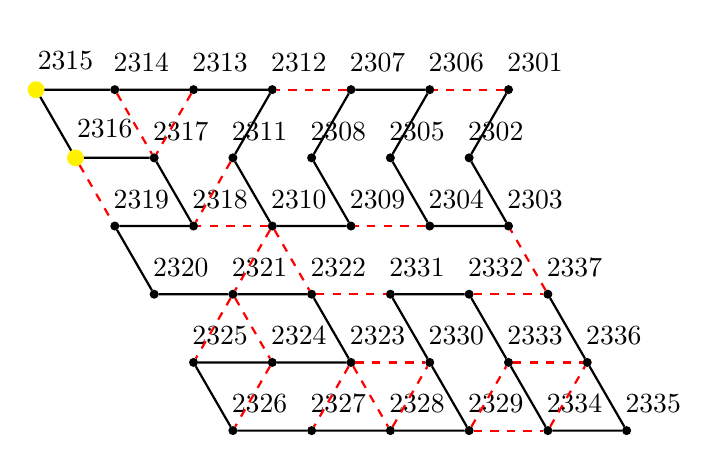
\begin{tikzpicture}[node distance=1cm,every node/.style={draw,circle,fill,inner sep=1pt}]
  \node (26) at (0:0)[label=above right:2326]{};
  \node (25) at (120:1)[label=above right:2325]{};
  \node (20)at (120:2)[label=above right:2320]{};
\node (19)at (120:3)[label=above right:2319]{};
\node [yellow,inner sep = 2pt] (16)at (120:4)[label=above right:2316]{};
\node [yellow,inner sep = 2pt] (15)at (120:5)[label=above right:2315]{};
  
\node[right of =15](14)[label=above right:2314]{};
\node[right of =14](13)[label=above right:2313]{};
\node[right of =13](12)[label=above right:2312]{};
\node[right of =12](7)[label=above right:2307]{};
\node[right of =7](6)[label=above right:2306]{};
\node[right of =6](1)[label=above right:2301]{};

\node[right of =16](17)[label=above right:2317]{};
\node[right of =17](11)[label=above right:2311]{};
\node[right of =11](8)[label=above right:2308]{};
\node[right of =8](5)[label=above right:2305]{};
\node[right of =5](2)[label=above right:2302]{};

\node[right of =19](18)[label=above right:2318]{};
\node[right of =18](10)[label=above right:2310]{};
\node[right of =10](9)[label=above right:2309]{};
\node[right of =9](4)[label=above right:2304]{};
\node[right of =4](3)[label=above right:2303]{};

\node[right of =20](21)[label=above right:2321]{};
\node[right of =21](22)[label=above right:2322]{};
\node[right of =22](31)[label=above right:2331]{};
\node[right of =31](32)[label=above right:2332]{};
\node[right of =32](37)[label=above right:2337]{};

\node[right of =25](24)[label=above right:2324]{};
\node[right of =24](23)[label=above right:2323]{};
\node[right of =23](30)[label=above right:2330]{};
\node[right of =30](33)[label=above right:2333]{};
\node[right of =33](36)[label=above right:2336]{};

\node[right of =26](27)[label=above right:2327]{};
\node[right of =27](28)[label=above right:2328]{};
\node[right of =28](29)[label=above right:2329]{};
\node[right of =29](34)[label=above right:2334]{};
\node[right of =34](35)[label=above right:2335]{};

  %\foreach \x in {1,2,...,35} \draw (\x)--(\abvance \x by 1);
  \draw[thick](1)--(2)--(3)--(4)--(5)--(6)--(7)--(8)--(9)--(10)--(11)--(12)--(13)--(14)--(15)--(16)--(17)--(18)--(19)--(20)--
(21)--(22)--(23)--(24)--(25)--(26)--(27)--(28)--(29)--(30)--(31)--(32)--(33)--(34)--(35)--(36)--(37);
\draw[dashed,thick,red](1)--(6);
\draw[dashed,thick,red](4)--(9);
\draw[dashed,thick,red](7)--(12);
\draw[dashed,thick,red](13)--(17);
\draw[dashed,thick,red](14)--(17);
\draw[dashed,thick,red](16)--(19);
\draw[dashed,thick,red](10)--(18);
\draw[dashed,thick,red](11)--(18);
\draw[dashed,thick,red](10)--(21);
\draw[dashed,thick,red](10)--(22);
\draw[dashed,thick,red](21)--(24);
\draw[dashed,thick,red](21)--(25);
\draw[dashed,thick,red](24)--(26);
\draw[dashed,thick,red](23)--(27);
\draw[dashed,thick,red](23)--(28);
\draw[dashed,thick,red](23)--(30);
\draw[dashed,thick,red](28)--(30);
\draw[dashed,thick,red](22)--(31);
\draw[dashed,thick,red](29)--(33);
\draw[dashed,thick,red](29)--(34);
\draw[dashed,thick,red](34)--(36);
\draw[dashed,thick,red](33)--(36);
\draw[dashed,thick,red](32)--(37);
\draw[dashed,thick,red](37)--(3);
  \end{tikzpicture}
  }
  %\caption*{横からの情報が0のときの折りたたみ}
  \end{minipage}

\begin{minipage}{0.2\hsize}
  \centering
  \scalebox{0.45}{
  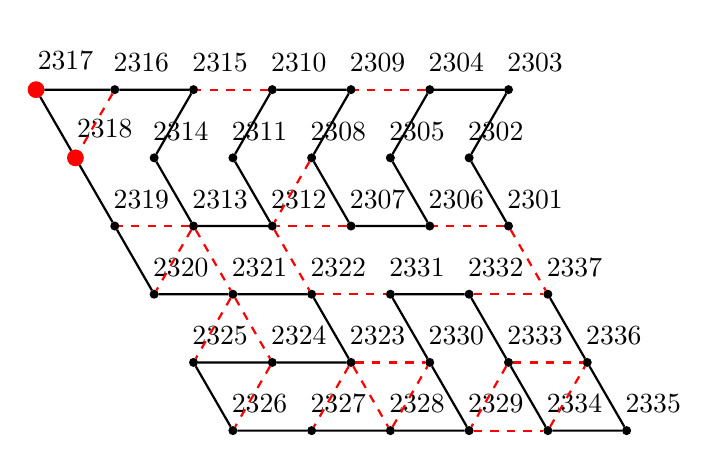
\begin{tikzpicture}[node distance=1cm,every node/.style={draw,circle,fill,inner sep=1pt}]
  \node (26) at (0:0)[label=above right:2326]{};
  \node (25) at (120:1)[label=above right:2325]{};
  \node (20)at (120:2)[label=above right:2320]{};
\node (19)at (120:3)[label=above right:2319]{};
\node [red,inner sep = 2pt] (18)at (120:4)[label=above right:2318]{};
\node [red,inner sep = 2pt] (17)at (120:5)[label=above right:2317]{};
  

\node[right of =19](13)[label=above right:2313]{};
\node[right of =13](12)[label=above right:2312]{};
\node[right of =12](7)[label=above right:2307]{};
\node[right of =7](6)[label=above right:2306]{};
\node[right of =6](1)[label=above right:2301]{};


\node[right of =18](14)[label=above right:2314]{};
\node[right of =14](11)[label=above right:2311]{};
\node[right of =11](8)[label=above right:2308]{};
\node[right of =8](5)[label=above right:2305]{};
\node[right of =5](2)[label=above right:2302]{};

\node[right of =17](16)[label=above right:2316]{};
\node[right of =16](15)[label=above right:2315]{};
\node[right of =15](10)[label=above right:2310]{};
\node[right of =10](9)[label=above right:2309]{};
\node[right of =9](4)[label=above right:2304]{};
\node[right of =4](3)[label=above right:2303]{};

\node[right of =20](21)[label=above right:2321]{};
\node[right of =21](22)[label=above right:2322]{};
\node[right of =22](31)[label=above right:2331]{};
\node[right of =31](32)[label=above right:2332]{};
\node[right of =32](37)[label=above right:2337]{};

\node[right of =25](24)[label=above right:2324]{};
\node[right of =24](23)[label=above right:2323]{};
\node[right of =23](30)[label=above right:2330]{};
\node[right of =30](33)[label=above right:2333]{};
\node[right of =33](36)[label=above right:2336]{};

\node[right of =26](27)[label=above right:2327]{};
\node[right of =27](28)[label=above right:2328]{};
\node[right of =28](29)[label=above right:2329]{};
\node[right of =29](34)[label=above right:2334]{};
\node[right of =34](35)[label=above right:2335]{};

  %\foreach \x in {1,2,...,35} \draw (\x)--(\abvance \x by 1);
  \draw[thick](1)--(2)--(3)--(4)--(5)--(6)--(7)--(8)--(9)--(10)--(11)--(12)--(13)--(14)--(15)--(16)--(17)--(18)--(19)--(20)--
(21)--(22)--(23)--(24)--(25)--(26)--(27)--(28)--(29)--(30)--(31)--(32)--(33)--(34)--(35)--(36)--(37);
\draw[dashed,thick,red](1)--(6);
\draw[dashed,thick,red](4)--(9);
\draw[dashed,thick,red](7)--(12);
\draw[dashed,thick,red](10)--(15);
\draw[dashed,thick,red](16)--(18);
\draw[dashed,thick,red](13)--(19);
\draw[dashed,thick,red](13)--(20);
\draw[dashed,thick,red](13)--(21);
\draw[dashed,thick,red](12)--(22);
\draw[dashed,thick,red](8)--(12);
\draw[dashed,thick,red](21)--(24);
\draw[dashed,thick,red](21)--(25);
\draw[dashed,thick,red](24)--(26);
\draw[dashed,thick,red](23)--(27);
\draw[dashed,thick,red](23)--(28);
\draw[dashed,thick,red](23)--(30);
\draw[dashed,thick,red](28)--(30);
\draw[dashed,thick,red](22)--(31);
\draw[dashed,thick,red](33)--(29);
\draw[dashed,thick,red](29)--(34);
\draw[dashed,thick,red](34)--(36);
\draw[dashed,thick,red](33)--(36);
\draw[dashed,thick,red](32)--(37);
\draw[dashed,thick,red](1)--(37);
  \end{tikzpicture}
  }
  %\caption*{横からの情報が1のときの折りたたみ}
  \end{minipage}
%  \end{tabular}
%  \caption{turn-lgp}
%\label{turn-lgp}
%\end{figure}
\begin{minipage}{0.1\hsize}
\ \\
\end{minipage}
%\begin{figure}[H]
%  \begin{tabular}{c}
  \begin{minipage}{0.2\hsize}
  \centering
  \scalebox{0.45}{
  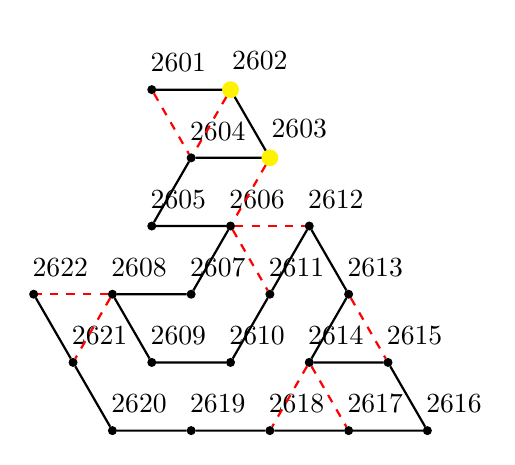
\begin{tikzpicture}[node distance=1cm,every node/.style={draw,circle,fill,inner sep=1pt}]
   \node (16) at (0:0)[label=above right:2616]{};
  \node (15) at (120:1)[label=above right:2615]{};
  \node (13)at (120:2)[label=above right:2613]{};
\node (12)at (120:3)[label=above right:2612]{};
\node [yellow,inner sep = 2pt] (3)at (120:4)[label=above right:2603]{};
\node [yellow,inner sep = 2pt] (2)at (120:5)[label=above right:2602]{};

  \node[left of =2](1)[label=above right:2601]{};
  \node[left of =3](4)[label=above right:2604]{};

  \node[left of =12](6)[label=above right:2606]{};
  \node[left of =6](5)[label=above right:2605]{};

  \node[left of =13](11)[label=above right:2611]{};
  \node[left of =11](7)[label=above right:2607]{};
  \node[left of =7](8)[label=above right:2608]{};
  \node[left of =8](22)[label=above right:2622]{};

  \node[left of =15](14)[label=above right:2614]{};
  \node[left of =14](10)[label=above right:2610]{};
  \node[left of =10](9)[label=above right:2609]{};
  \node[left of =9](21)[label=above right:2621]{};
  
\node[left of =16](17)[label=above right:2617]{};
  \node[left of =17](18)[label=above right:2618]{};
  \node[left of =18](19)[label=above right:2619]{};
  \node[left of =19](20)[label=above right:2620]{};
  \draw[thick](1)--(2)--(3)--(4)--(5)--(6)--(7)--(8)--(9)--(10)--(11)--(12)--(13)--(14)--(15)--(16)--(17)--(18)--(19)--(20)--
(21)--(22);
\draw[dashed,thick,red](1)--(4);
\draw[dashed,thick,red](2)--(4);
\draw[dashed,thick,red](3)--(6);
\draw[dashed,thick,red](6)--(12);
\draw[dashed,thick,red](6)--(11);
\draw[dashed,thick,red](8)--(22);
\draw[dashed,thick,red](8)--(21);
\draw[dashed,thick,red](13)--(15);
\draw[dashed,thick,red](14)--(17);
\draw[dashed,thick,red](14)--(18);
  \end{tikzpicture}
  }
  %\caption*{横からの情報が0のときの折りたたみ}
  \end{minipage}

\begin{minipage}{0.2\hsize}
  \centering
  \scalebox{0.45}{
  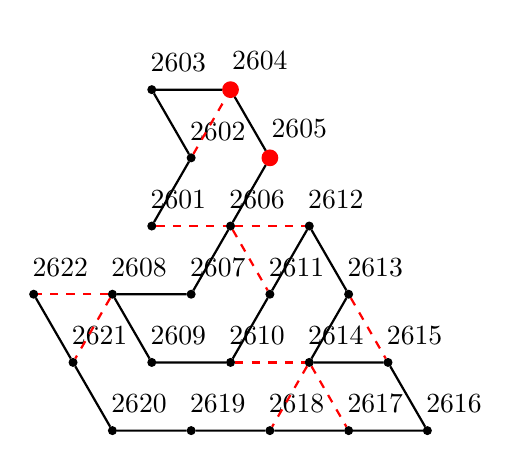
\begin{tikzpicture}[node distance=1cm,every node/.style={draw,circle,fill,inner sep=1pt}]
  \node (16) at (0:0)[label=above right:2616]{};
  \node (15) at (120:1)[label=above right:2615]{};
  \node (13)at (120:2)[label=above right:2613]{};
\node (12)at (120:3)[label=above right:2612]{};
\node [red,inner sep = 2pt] (5)at (120:4)[label=above right:2605]{};
\node [red,inner sep = 2pt] (4)at (120:5)[label=above right:2604]{};

  \node[left of =4](3)[label=above right:2603]{};
  \node[left of =5](2)[label=above right:2602]{};

  \node[left of =12](6)[label=above right:2606]{};
  \node[left of =6](1)[label=above right:2601]{};

  \node[left of =13](11)[label=above right:2611]{};
  \node[left of =11](7)[label=above right:2607]{};
  \node[left of =7](8)[label=above right:2608]{};
  \node[left of =8](22)[label=above right:2622]{};

  \node[left of =15](14)[label=above right:2614]{};
  \node[left of =14](10)[label=above right:2610]{};
  \node[left of =10](9)[label=above right:2609]{};
  \node[left of =9](21)[label=above right:2621]{};
  
\node[left of =16](17)[label=above right:2617]{};
  \node[left of =17](18)[label=above right:2618]{};
  \node[left of =18](19)[label=above right:2619]{};
  \node[left of =19](20)[label=above right:2620]{};
  \draw[thick](1)--(2)--(3)--(4)--(5)--(6)--(7)--(8)--(9)--(10)--(11)--(12)--(13)--(14)--(15)--(16)--(17)--(18)--(19)--(20)--
(21)--(22);
\draw[dashed,thick,red](2)--(4);
\draw[dashed,thick,red](1)--(6);
\draw[dashed,thick,red](6)--(12);
\draw[dashed,thick,red](6)--(11);
\draw[dashed,thick,red](8)--(22);
\draw[dashed,thick,red](8)--(21);
\draw[dashed,thick,red](10)--(14);
\draw[dashed,thick,red](13)--(15);
\draw[dashed,thick,red](14)--(17);
\draw[dashed,thick,red](14)--(18);
  \end{tikzpicture}
  }
  %\caption*{横からの情報が1のときの折りたたみ}
  \end{minipage}

  \end{tabular}
  \caption{left:turn-lgp,right:turn-rgp}
\label{square-square}
\end{figure}


%--------------------------------------------


\begin{figure}[H]
  \begin{tabular}{c}
 
  
  \begin{minipage}{0.5\hsize}
  \centering
  \scalebox{0.5}{
  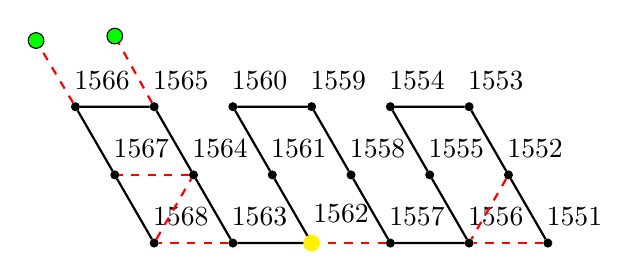
\begin{tikzpicture}[node distance=1cm,every node/.style={draw,circle,fill,inner sep=1pt}]
   \node (1) at (0:0)[label=above right:1551]{};
  \node (2) at (120:1)[label=above right:1552]{};
  \node (3)at (120:2)[label=above right:1553]{};
  \node[left of= 1] (6) [label=above right:1556]{};
  \node[left of =6](7)[label=above right:1557]{};
  \node[left of =7,yellow,inner sep = 2pt](12)[label=above right:1562]{};
\node[left of =12](13)[label=above right:1563]{};
\node[left of =13](18)[label=above right:1568]{};
  \node[left of =2](5)[label=above right:1555]{};
  \node[left of =5](8)[label=above right:1558]{};
  \node[left of =8](11)[label=above right:1561]{};
\node[left of =11](14)[label=above right:1564]{};
\node[left of =14](17)[label=above right:1567]{};
  \node[left of =3](4)[label=above right:1554]{};
  \node[left of =4](9)[label=above right:1559]{};
  \node[left of =9](10)[label=above right:1560]{};
\node[left of =10](15)[label=above right:1565]{};
\node[left of =15](16)[label=above right:1566]{};
\coordinate[left of = 17](99){};
\node[above =1.6cm of  17,fill = green,inner sep = 2pt](100){};
\node[above =1.6cm of  99,fill = green,inner sep = 2pt](101){};
  \draw[thick](1)--(2)--(3)--(4)--(5)--(6)--(7)--(8)--(9)--(10)--(11)--(12)--(13)--(14)--(15)--(16)--(17)--(18);
  \draw[dashed,thick,red](1)--(6);
  \draw[dashed,thick,red](2)--(6);
\draw[dashed,thick,red](7)--(12);
\draw[dashed,thick,red](13)--(18);
\draw[dashed,thick,red](18)--(14);
\draw[dashed,thick,red](14)--(17);
\draw[dashed,thick,red](16)--(101);
\draw[dashed,thick,red](15)--(100);
  \end{tikzpicture}
  }
  \end{minipage}

 \begin{minipage}{0.5\hsize}
  \centering
  \scalebox{0.5}{
  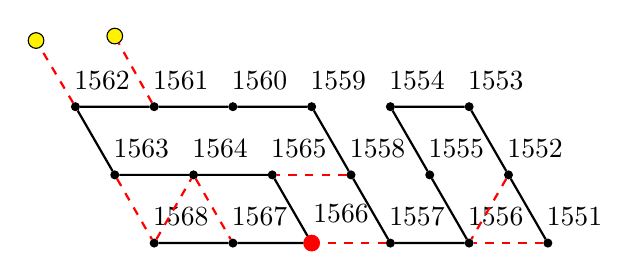
\begin{tikzpicture}[node distance=1cm,every node/.style={draw,circle,fill,inner sep=1pt}]
   \node (1) at (0:0)[label=above right:1551]{};
  \node (2) at (120:1)[label=above right:1552]{};
  \node (3)at (120:2)[label=above right:1553]{};
  \node[left of= 1] (6) [label=above right:1556]{};
  \node[left of =6](7)[label=above right:1557]{};
  \node[left of =7,red,inner sep = 2pt](16)[label=above right:1566]{};
\node[left of =16](17)[label=above right:1567]{};
\node[left of =17](18)[label=above right:1568]{};
  \node[left of =2](5)[label=above right:1555]{};
  \node[left of =5](8)[label=above right:1558]{};
  \node[left of =8](15)[label=above right:1565]{};
\node[left of =15](14)[label=above right:1564]{};
\node[left of =14](13)[label=above right:1563]{};
  \node[left of =3](4)[label=above right:1554]{};
  \node[left of =4](9)[label=above right:1559]{};
  \node[left of =9](10)[label=above right:1560]{};
\node[left of =10](11)[label=above right:1561]{};
\node[left of =11](12)[label=above right:1562]{};
\coordinate[left of = 13](99){};
\node[above =1.6cm of  13,fill = yellow,inner sep = 2pt](100){};
\node[above =1.6cm of  99,fill = yellow,inner sep = 2pt](101){};
  \draw[thick](1)--(2)--(3)--(4)--(5)--(6)--(7)--(8)--(9)--(10)--(11)--(12)--(13)--(14)--(15)--(16)--(17)--(18);
  \draw[dashed,thick,red](1)--(6);
\draw[dashed,thick,red](2)--(6);
\draw[dashed,thick,red](8)--(15);
\draw[dashed,thick,red](7)--(16);
\draw[dashed,thick,red](13)--(18);
\draw[dashed,thick,red](18)--(14);
\draw[dashed,thick,red](14)--(17);
\draw[dashed,thick,red](12)--(101);
\draw[dashed,thick,red](11)--(100);
  \end{tikzpicture}
  }
  \end{minipage}
 
 \end{tabular}
  \caption{The possible two conformations of move.}
\label{move}
\end{figure} 
%
%\begin{figure}[H]
%  \begin{tabular}{c}
% 
%  
% 
%
% \begin{minipage}{0.5\hsize}
%  \centering
%  \scalebox{0.5}{
%  \begin{tikzpicture}[node distance=1cm,every node/.style={draw,circle,fill,inner sep=1pt}]
%  \node [red,inner sep = 2pt] (13) at (0:0)[label=above right:13]{};
%  \node (12) at (120:1)[label=above right:12]{};
%  \node (1)at (120:2)[label=above right:1]{};
%  \node[right of= 1] (2) [label=above right:2]{};
%  \node[right of =2](3)[label=above right:3]{};
%  \node[right of =3](4)[label=above right:4]{};
%  \node[right of =4](5)[label=above right:5]{};
%  \node[right of =5](6)[label=above right:6]{};
%  \node[right of =10](9)[label=above right:9]{};
%  \node[right of =9](8)[label=above right:8]{};
%  \node[right of =8](7)[label=above right:7]{};
%  
%  \node[right of =16](17)[label=above right:17]{};
%  \node[right of =11](10)[label=above right:10]{};
%  \node[right of =12](11)[label=above right:11]{};
%  \node[right of =13](14)[label=above right:14]{};
%  \node[right of =14](15)[label=above right:15]{};
%  \node[right of =15](16)[label=above right:16]{};
%\node[right of =17](18)[label=above right:18]{};
%\node[above =1.6cm of 11,fill = green,inner sep = 2pt](100){};
%  \draw(1)--(2)--(3)--(4)--(5)--(6)--(7)--(8)--(9)--(10)--(11)--(12)--(13)--(14)--(15)--(16)--(17)--(18);
%  \end{tikzpicture}
%  }
%  %%\caption*{1を下に送る折りたたみ}
%  \end{minipage}
%  \end{tabular}
%  \caption{%body-lpx2
%change-routes}
%\label{body-lpx2}
%\end{figure} 

%\begin{figure}[H]
%  \begin{tabular}{c}
% \begin{minipage}{0\hsize}
%  \centering
%  \scalebox{0.45}{
%  \begin{tikzpicture}[node distance=1cm,every node/.style={draw,circle,fill,inner sep=1pt}]
%  \node [red,inner sep = 2pt] (13) at (0:0)[label=above right:13]{};
%  \node (12) at (120:1)[label=above right:12]{};
%  \node (1)at (120:2)[label=above right:1]{};
%  \node[left of= 1] (2) [label=above right:2]{};
%  \node[left of =2](3)[label=above right:3]{};
%  \node[left of =3](4)[label=above right:4]{};
%  \node[left of =4](5)[label=above right:5]{};
%  \node[left of =5](6)[label=above right:6]{};
%  \node[left of =10](9)[label=above right:9]{};
%  \node[left of =9](8)[label=above right:8]{};
%  \node[left of =8](7)[label=above right:7]{};
%  
%  \node[left of =16](17)[label=above right:17]{};
%  \node[left of =11](10)[label=above right:10]{};
%  \node[left of =12](11)[label=above right:11]{};
%  \node[left of =13](14)[label=above right:14]{};
%  \node[left of =14](15)[label=above right:15]{};
%  \node[left of =15](16)[label=above right:16]{};
%\node[left of =17](18)[label=above right:18]{};
%\node[above =1.6cm of 11,fill = green,inner sep = 2pt](100){};
%  \draw(1)--(2)--(3)--(4)--(5)--(6)--(7)--(8)--(9)--(10)--(11)--(12)--(13)--(14)--(15)--(16)--(17)--(18);
%  \end{tikzpicture}
%  }
%  %\caption*{横からの情報が0のときの折りたたみ}
%  \end{minipage}
%
%
%
%  \end{tabular}
%  \caption{change_route}
%\label{square-square}
%\end{figure}
\end{document}